
\documentclass[final]{beamer}

\usepackage[scale=1.24]{beamerposter} % Use the beamerposter package for laying out the poster
\usepackage{ragged2e}

\usetheme{confposter} % Use the confposter theme supplied with this template

\setbeamercolor{block title}{fg=ngreen,bg=white} % Colors of the block titles
\setbeamercolor{block body}{fg=black,bg=white} % Colors of the body of blocks
\setbeamercolor{block alerted title}{fg=white,bg=dblue!70} % Colors of the highlighted block titles
\setbeamercolor{block alerted body}{fg=black,bg=dblue!10} % Colors of the body of highlighted blocks
% Many more colors are available for use in beamerthemeconfposter.sty

%-----------------------------------------------------------
% Define the column widths and overall poster size
% To set effective sepwid, onecolwid and twocolwid values, first choose how many columns you want and how much separation you want between columns
% In this template, the separation width chosen is 0.024 of the paper width and a 4-column layout
% onecolwid should therefore be (1-(# of columns+1)*sepwid)/# of columns e.g. (1-(4+1)*0.024)/4 = 0.22
% Set twocolwid to be (2*onecolwid)+sepwid = 0.464
% Set threecolwid to be (3*onecolwid)+2*sepwid = 0.708

\newlength{\sepwid}
\newlength{\onecolwid}
\newlength{\twocolwid}
\newlength{\threecolwid}
\setlength{\paperwidth}{48in} % A0 width: 46.8in
\setlength{\paperheight}{36in} % A0 height: 33.1in
\setlength{\sepwid}{0.024\paperwidth} % Separation width (white space) between columns
\setlength{\onecolwid}{0.22\paperwidth} % Width of one column
\setlength{\twocolwid}{0.464\paperwidth} % Width of two columns
\setlength{\threecolwid}{0.708\paperwidth} % Width of three columns
\setlength{\topmargin}{-0.5in} % Reduce the top margin size
%-----------------------------------------------------------

\usepackage{graphicx}  % Required for including images

\usepackage{booktabs} % Top and bottom rules for tables

%----------------------------------------------------------------------------------------
%	TITLE SECTION 
%----------------------------------------------------------------------------------------

\title{X-Prod: Efficient and Scalable Cartesian Product distribution} % Poster title

\author{
Gopal Vijayaraghavan, Zhiyuan Yang, Hitesh Shah \\ 
\{gopalv,zhiyuany,hitesh\}@apache.org
} % Author(s)

\institute{Apache Tez} % Institution(s)

%----------------------------------------------------------------------------------------

\begin{document}

\addtobeamertemplate{block end}{}{\vspace*{2ex}} % White space under blocks
\addtobeamertemplate{block alerted end}{}{\vspace*{2ex}} % White space under highlighted (alert) blocks

\setlength{\belowcaptionskip}{2ex} % White space under figures
\setlength\belowdisplayshortskip{2ex} % White space under equations

\begin{frame}[t] % The whole poster is enclosed in one beamer frame

\begin{columns}[t] % The whole poster consists of three major columns, the second of which is split into two columns twice - the [t] option aligns each column's content to the top

\begin{column}{\sepwid}\end{column} % Empty spacer column

\begin{column}{\onecolwid} % The first column

%----------------------------------------------------------------------------------------
%	OBJECTIVES
%----------------------------------------------------------------------------------------

\begin{alertblock}{Apache Tez}
Apache Tez is a DAG processing engine built on top of Apache Hadoop YARN. It offers
\begin{itemize}
\item Performance gains over Map Reduce 
\item Low level dataflow APIs
\item Plugin architecture for control plane
\item Dynamic physical flow decisions
\item Plan reconfiguration at runtime 
\end{itemize}

\end{alertblock}

%----------------------------------------------------------------------------------------
%	QUICK REVISION
%----------------------------------------------------------------------------------------

\begin{block}{Cartesian Product Problems}
%\textbf{Problems which generate cross-products}
%\begin{itemize}
%\item {Non-equality $\Theta$-joins} 
%\item {Geographical containment} 
%\item {Genome Edit distance} 
%\item {BiTemporal overlaps}
%\end{itemize}
\textbf{Non-equality Theta Joins}:
Theta joins are generalized joins which require a sub-set of cross-product to be selected by 
a non-equality like \texttt{a <> b} or a complex condition like \texttt{suspect = seller or suspect = buyer}.

\textbf{Geographical containment}:
Geographical containment conditions like \texttt{ST\_Contains(area, point)} are expressed as cross-products with filters in the absence of spatial indices.

\textbf{Genome Edit distance}:
Computing edit distance values of all elements within a large set and filtering them for similarity requires a cross-product distribution. This can 
be expressed as a cross join with a join condition which could distance by executing \texttt{LevenshteinDistance(a,b) <= n}.

\textbf{BiTemporal Overlaps}:
Industrial IoT historian tools utilize BiTemporal tables which allow for compression of values and the metric system to evolve over time, by storing a
tuple like \texttt{(from, to, identifier, metric, value)} to indicate steady state during a time period.
Processing these data streams to answer complex queries such as \textit{"what was the altitude when the RPM was above X and the temperature was above Y"}
generates self cross-products with \texttt{OVERLAPS(period1, period2)} to generate the wide steady-state table.
\end{block}

%----------------------------------------------------------------------------------------

\end{column} % End of the first column

\begin{column}{\sepwid}\end{column} % Empty spacer column

\begin{column}{\twocolwid} % Begin a column which is two columns wide (column 2)

\begin{columns}[t,totalwidth=\twocolwid] % Split up the two columns wide column

\begin{column}{\onecolwid}\vspace{-.6in} % The first column within column 2 (column 2.1)

%----------------------------------------------------------------------------------------
%	MATERIALS
%----------------------------------------------------------------------------------------

\begin{block}{Map Reduce \& Shuffle}

Map Reduce has a Shuffle operation that naturally produces a hash distribution useful for equi-joins.

\begin{figure}
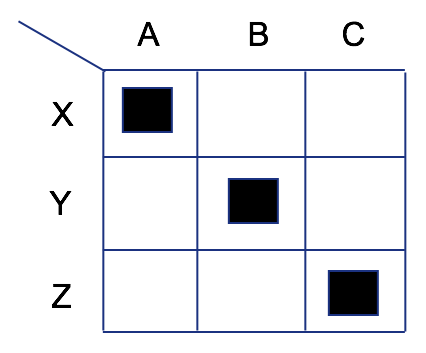
\includegraphics{figures/mr-shuffle.png}
\end{figure}

\end{block}

%----------------------------------------------------------------------------------------

\end{column} % End of column 2.1

\begin{column}{\onecolwid}\vspace{-.6in} % The second column within column 2 (column 2.2)

%----------------------------------------------------------------------------------------
%	P
%----------------------------------------------------------------------------------------

\begin{block}{Tez \& Shuffle}

Tez can define the distribution function to produce a full product of data partitions.

\begin{figure}
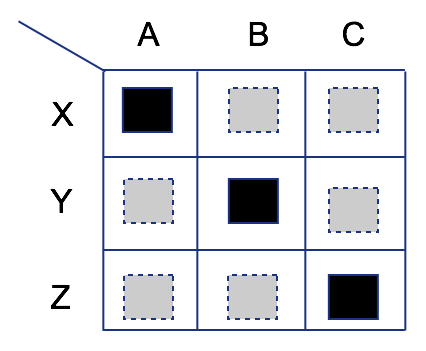
\includegraphics{figures/X-prod-1.png}
\end{figure}

\end{block}

%----------------------------------------------------------------------------------------

\end{column} % End of column 2.2

\end{columns} % End of the split of column 2 - any content after this will now take up 2 columns width

%----------------------------------------------------------------------------------------
%	IMPORTANT To REMEMBER
%----------------------------------------------------------------------------------------

\begin{alertblock}{Tez: EdgeManager plugins}

Where Map Reduce comes with a single configuration for the Shuffle Edge between Map \& Reduce vertices,
Tez makes the Edge as a routing layer for \texttt{DataMovementEvent}, which can be duplicated
between tasks or multiplexed multiple events to one task.

\end{alertblock} 

%----------------------------------------------------------------------------------------

\begin{columns}[t,totalwidth=\twocolwid] % Split up the two columns wide column again

\begin{column}{\onecolwid} % The first column within column 2 (column 2.1)

%----------------------------------------------------------------------------------------
% Tez Cross-product #1	
%----------------------------------------------------------------------------------------

\begin{block}{Map-Reduce: Synthetic Join}

\begin{figure}
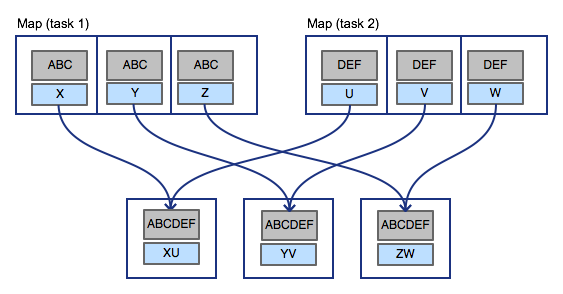
\includegraphics{figures/gfcross.png}
\end{figure}

Map-Reduce can effectively produce a join on synthetic keys and force the hash distribution
function to do a cross-product distribution. This duplicates the data on the 
source side, which makes increased parallelism for destination tasks more expensive.
Tez can produce the same destination distribution without the data repetition, by generating 
${N}^2$ events for shuffle.

\end{block}

%----------------------------------------------------------------------------------------

\end{column} % End of column 2.1

\begin{column}{\onecolwid} % The second column within column 2 (column 2.2)

%----------------------------------------------------------------------------------------
%	PROOF OF VIETA'S FORMULAS
%----------------------------------------------------------------------------------------

\begin{block}{Tez: X-Product}


\begin{figure}
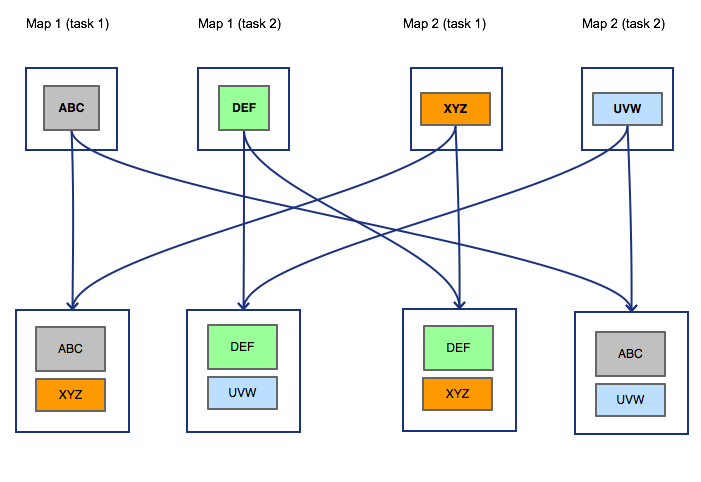
\includegraphics{figures/Tez-XProd-1.png}
\end{figure}

The fundamental disadvantage of a product of shuffle partitions is that to produce ${N}^2$ reduce tasks,
there are N data partitions from each source task, which incurs a large number of random seek IO operations.
The \texttt{DataMovementEvent} routing pattern allows Tez to avoid that and produce a product of the source
task indices to produce parallelism for the reducers without splitting up the output of the map-tasks.

\end{block}


%----------------------------------------------------------------------------------------

\end{column} % End of column 2.2

\end{columns} % End of the split of column 2

\end{column} % End of the second column

\begin{column}{\sepwid}\end{column} % Empty spacer column

\begin{column}{\onecolwid} % The third column

%----------------------------------------------------------------------------------------
%	CONCLUSION
%----------------------------------------------------------------------------------------

\begin{block}{Tez: Skewed X-Product}

\begin{figure}
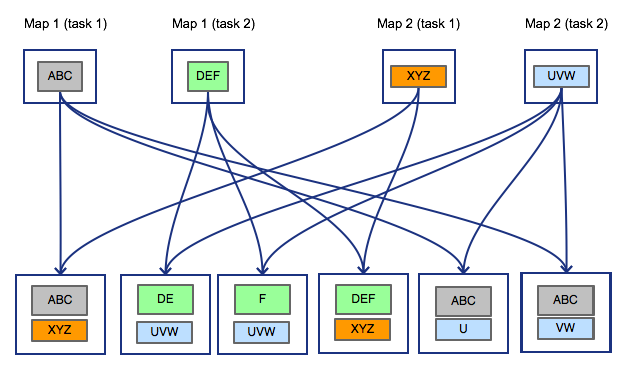
\includegraphics{figures/Tez-XProd-2.png}
\end{figure}

The presence of input skew into the Cross Product can result in uneven distribution to the reducers, this can be
mitigated by writing partitioned output from each source task and merging adjacent partitions using size information
encoded into the \texttt{DataMovementEvent}. This removes the random seeks when the reads are merged, but it can group
across partitions and tasks at the same time.

\end{block}

%----------------------------------------------------------------------------------------
%	ACKNOWLEDGEMENTS
%----------------------------------------------------------------------------------------

%\setbeamercolor{block title}{fg=red,bg=white} % Change the block title color

\begin{block}{Tez: Fair Grouping}

\begin{figure}
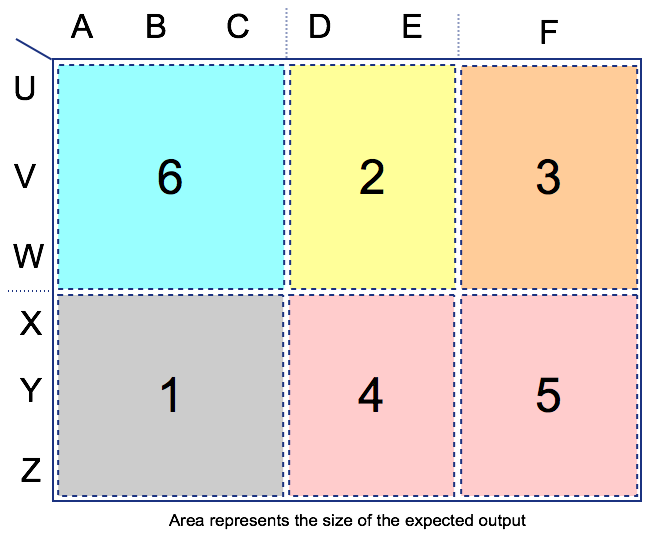
\includegraphics{figures/Data-Grouping.png}
\end{figure}

From the data-size information contained in the \texttt{DataMovementEvent}, the Edge can try to 
avoid skewed destination tasks by grouping together adjacent regions conditionally, to produce 
tasks of similar sizes. Fairness computation today is heuristic based and does not wait for 
perfect information to start scheduling downstream tasks.
\end{block}

%----------------------------------------------------------------------------------------

\end{column} % End of the third column

\end{columns} % End of all the columns in the poster

\end{frame} % End of the enclosing frame

\end{document}
